This chapter describes the process of desigining the molecule chip experiment.
This was motivated by three main factors: the need to integrate with the
existing experiment, the core proposal of confining molecules close to a
microwave guide, and the practicalities of fabricating the chip. Here I will
focus on how the first two factors informed the design choices, with changes
due to fabrication discussed in chapter~\ref{fab}. The design will be further
justified by simulation in chapter~\ref{sim}.

We begin with a discussion of
the existing experiment, and where the chip fits into it. I will then discuss
the process that lead us to choose a magnetic trap for our design. I will
present the final design \cm{and how it can be integrated with the existing
apparatus}. 

\section{Existing \CaF{} apparatus}

In this section I will present a summary of the process used to produce
ultracold \CaF{} molecules in a magnetic trap, which we intend to load onto the
chip trap. We will consider the various stages of the process, which is
presented in \myfigref{overview:fig:CaFcartoon}. First a beam of \CaF{}
molecules is created using a buffer gas
source~\cite{doi:10.1080/09500340.2017.1384516}. The beam is then slowed by
application of slowing light opposing its direction of
travel~\cite{Truppe2017a}. The slowing light can also be applied in the
transverse direction to reduce the broadening of the beam during its flight.
The molecules are captured in a MOT~\cite{Williams2017} and cooled in optical
molasses~\cite{Truppe2017} before being optically pumped into a weak field
seeking state~\cite{WilliamsMagnetic2018}. This allows for magnetic trapping
and transport of the molecules.

\begin{figure}
  \cm{TODO: Cartoon of CaF experiment up to MOT chamber}
  \caption{}
  \label{overview:fig:CaFcartoon}
\end{figure}

\subsection*{Buffer gas source}

In the buffer gas source, a copper cell containing a \cm{calcium} target is
cooled to \SI{4}{\kelvin}. \cm{Helium} (the eponymous buffer gas) flows into
the cell, thermalises with the cell walls and flows out through the exit
aperture. \cm{SF6} is also injected into the cell, and a high-power \cm{ndyag}
laser is fired at the target. The laser ablates the \cm{calcium} target,
producing \cm{Ca atoms} which react with the \cm{SF6} to produce \CaF{}
molecules which thermalise with the \cm{helium} and follow the flow out of the
exit aperture.  The result is a pulsed beam of \CaF{} molecules with typical
mean velocity \SI{160}{\meter\per\second}.

\subsection*{Slowing the beam}

The beam velocity can be further reduced by application of a counter-propagating
beam of slowing light. The light is resonant with the \cm{$X(v=0)\rightarrow
B$} transition \cm{($\mathcal{L^S_{00}}$}. A \SI{5}{\gauss} magnetic field is
applied, and the slowing light is linearly polarised at a relative
\SI{45}{\degree} angle, to remix dark ground states. The slowing light is
combined with repump light from \cm{$X(v=1)\rightarrow A(v=0)$, $\mathcal{L}_{10}$}
to avoid losing molecules that scatter into \cm{$X(v=1)$}. Since the molecules'
velocity will decrease during the slowing, the Doppler shift of the transition
frequency will also change. We account for this by chirping the slowing light,
and broadening the repump light. This process can reduce the molecule velocity
to \cm{??}.

\subsection*{Transverse cooling}

Slowing the beam has the undesirable effect of increasing the transverse
velocity of the molecules. This is due to the random walk of the molecules as
they scatter photons from the slowing light. To counteract this we apply
slowing beams in the transverse direction, also on the $\mathcal{L}_{00}^S$
transition. The slowing procedure described above is carried out
simultaneously, providing the remixing of dark ground states and the $v=1$
repump light.
%
Scattering of light in the transverse direction can collimate the beam, and has
been shown to improve the population of the MOT by a factor of $\sim3$. 

\subsection*{Capture in a MOT}

The \CaF{} beam travels \cm{some distance}, undergoing slowing and transverse
cooling before reaching the MOT chamber, where we capture the molecules. The
\CaF{} MOT is a type-II MOT~\cite{}, meaning that the angular momentum of the
excited state ($A(v=0)$, with $F'=1$) is greater than that of the ground state
($X(v=0)$ with $F=2$). Unlike a type-I MOT, it is therefore possible for a
molecule that has been pumped into the excited state to decay into a dark
state, or into a state that is anti-trapped by the MOT~\cite{}.

To resolve this, a dual-frequency MOT is employed. The main MOT transition is
addressed by the \pewpew{C}{00} light, with r.f.\ sidebands added to address
the different hyperfine levels. The sideband addressing the $F=1$ hyperfine
state is given opposite polarisation, and simultaneously serves as a second
frequency for the $F=2$ state, ensuring that the normally anti-trapped states
are repumped by the restoring beam into the MOT cycle. This is shown in \cm{a
figure}. The $F=2$ level is now strongly trapped and although the other levels
remain weakly trapped, this is sufficient to create a strong MOT.

The branching ratios of \CaF{} mean that the excited state can decay into
$X(v>0)$ states. One of the chief reasons that \CaF{} is chosen for our
experiment is that it has highly diagonal Franck-Condon factors, and so the
decay into these other states is minimised. However it is still essential to
repump the $X(v=1,2,3)$ states, which we do with the \pewpew{}{10}
\pewpew{}{21} and \pewpew{}{32} lasers respectively. Once again, r.f.\
sidebands are added to address the hyperfine levels of the $X$ state.

The capture velocity of the MOT is \cm{??} meaning that we are typically able
to capture $??$ molecules from our beam. The MOT population can be estimated by
looking at the scatter, or by turning off the light and performing
light-induced fluorescence imaging using \pewpew{C}{00}. The MOT temperature is
typically \cm{}, and this can be further reduced by lowering the intensity of
\pewpew{C}{00}~\cite{Truppe2017} \cm{what is final temp?}

\subsection*{Optical molasses}

Sub-Doppler cooling of \CaF{} is achievable by employing a blue-detuned
molasses. In this scheme the MOT coils are switched off, and \pewpew{C}{00}
is detuned to be blue-detuned \cm{by how much?}.  Consider the example of a
$F=1$ hyperfine level ground state, and $F=0$ excited state which is shown in
\cm{fig like Hannah's 5.1}. A polarisation gradient is established across the
molasses. In regions where the polarisation is $\sigma_-$ ($\sigma_-$) only the
$m=1$ ($m=-1$) ground state is coupled to the light.

The a.c.\ Stark shift now acts on the bright states, meaning that as they move
through the light field they lose kinetic energy. Near the peak of the energy
shift, the bright state molecules are preferentially pumped into the dark
state. Meanwhile the dark states will adiabatically transfer back to bright
states, which occurs preferentially at regions where the bright and dark states
are close in energy. This cycle then repeats, resulting in the molecule losing
energy as it passes through the light field.

% TODO Cite Molecules cooled belowo DOppler limit and
% Weidemu ̈ller, M., Esslinger, T., Ol’shanii, M. A., Hem- merich, A. & Ha ̈nsch, T. W. A novel scheme for efficient cooling below the photon recoil limit. EPL 27, 109–114 (1994).

In the \CaF{} experiment, the situation is not so simple. We must account for
intensity gradients as well as those of polarisation, and of course the real
experiment occurs in three dimensions not one. Details of this scheme can be
found in \inlineref{1367-2630-18-12-123017} and~\cite{Truppe2017}.

\subsection*{Magnetic trapping and transport}

\cm{inc. optical pumping}

\subsection*{Other experiments}
% TODO Is this section really necessary?

% TODO Rework this para? Maybe it just becomes a sentence, something like "we
% use this setup for lots of things, not we want to use it for chip instead"
The \CaF{} MOT is the workhorse of our experiment, providing molecules which
can be further cooled cooled further (as discussed above) used for experiments
in collisions with \Rb{} atoms (see \inlinerefs{Jurgilas2021, JurgilasIOP2021,
PhysRevLett.126.153401}) and optical tweezers. The tweezer experiment is
undertaken in the neighbouring tweezer chamber, which is loaded by transporting
molecules in a magnetic transport trap (MTT), a quadrupole trap with coils
mounted on a transport stage outside the vacuum chamber. This transport of the
molecules is similar to that used in
\inlinerefs{Lewandowski2003,PhysRevResearch.1.033035} and elsewhere, it will be
discussed further below and in \cm{transport chapter}.







\section{Design requirements}

%\begin{itemize}
%  \item Andr\'e proposal, want to strongly couple to coplanar waveguides
%  \item Want to do quantum operations with rotational stretched states
%  \item Need small size scale
%  \item Height limited by VdW force, as per Ed's notebook (Charles Smith also said something
%    about charges causing decoherence?) height gives scale size
%  \item We want to use magnetic trapping rather than electric (as explained
%    in QSUM report: long coherence times and easier to load (?))
%  \item Need to be able to load (one step is no good, ref. next chapter)
%\end{itemize}

As discussed in \cm{the introduction} the aim of this project is ultimately to
trap molecules in close proximity to microwave resonators so that we can
perform coherent control of quantum states on the rotational transitions in the
molecules.
%
Following the proposal by \inlineref{Andre2006}, this can be achieved in a chip
architecture, with the molecule trapped as close to the resonator as possible.
%
\cm{Calculation of VdW force to get the 10um figure}
%
Given that the molecules will be $\sim\SI{10}{\micro\meter}$ from the surface,
% TODO just smaller scale surely?
we will require that trapping electronics will be of a similar or smaller
scale for the trapping potential to keep the molecule \cm{well localised}.
Features of such a size can be easily created by standard photolithography
techniques.

Additionally, we aim to integrate into our existing chip experiment. This can
be done by the addition of a new chamber to our setup, shown in
\myfigref{overview:fig:vacuumsystem}. The chip chamber will be positioned along
the existing MTT axis, allowing extension of the transport system and the
delivery of molecules to this chamber. \CaF{} molecules can then be transferred
onto the chip trap.

\begin{figure}[htb]
  \centering
  %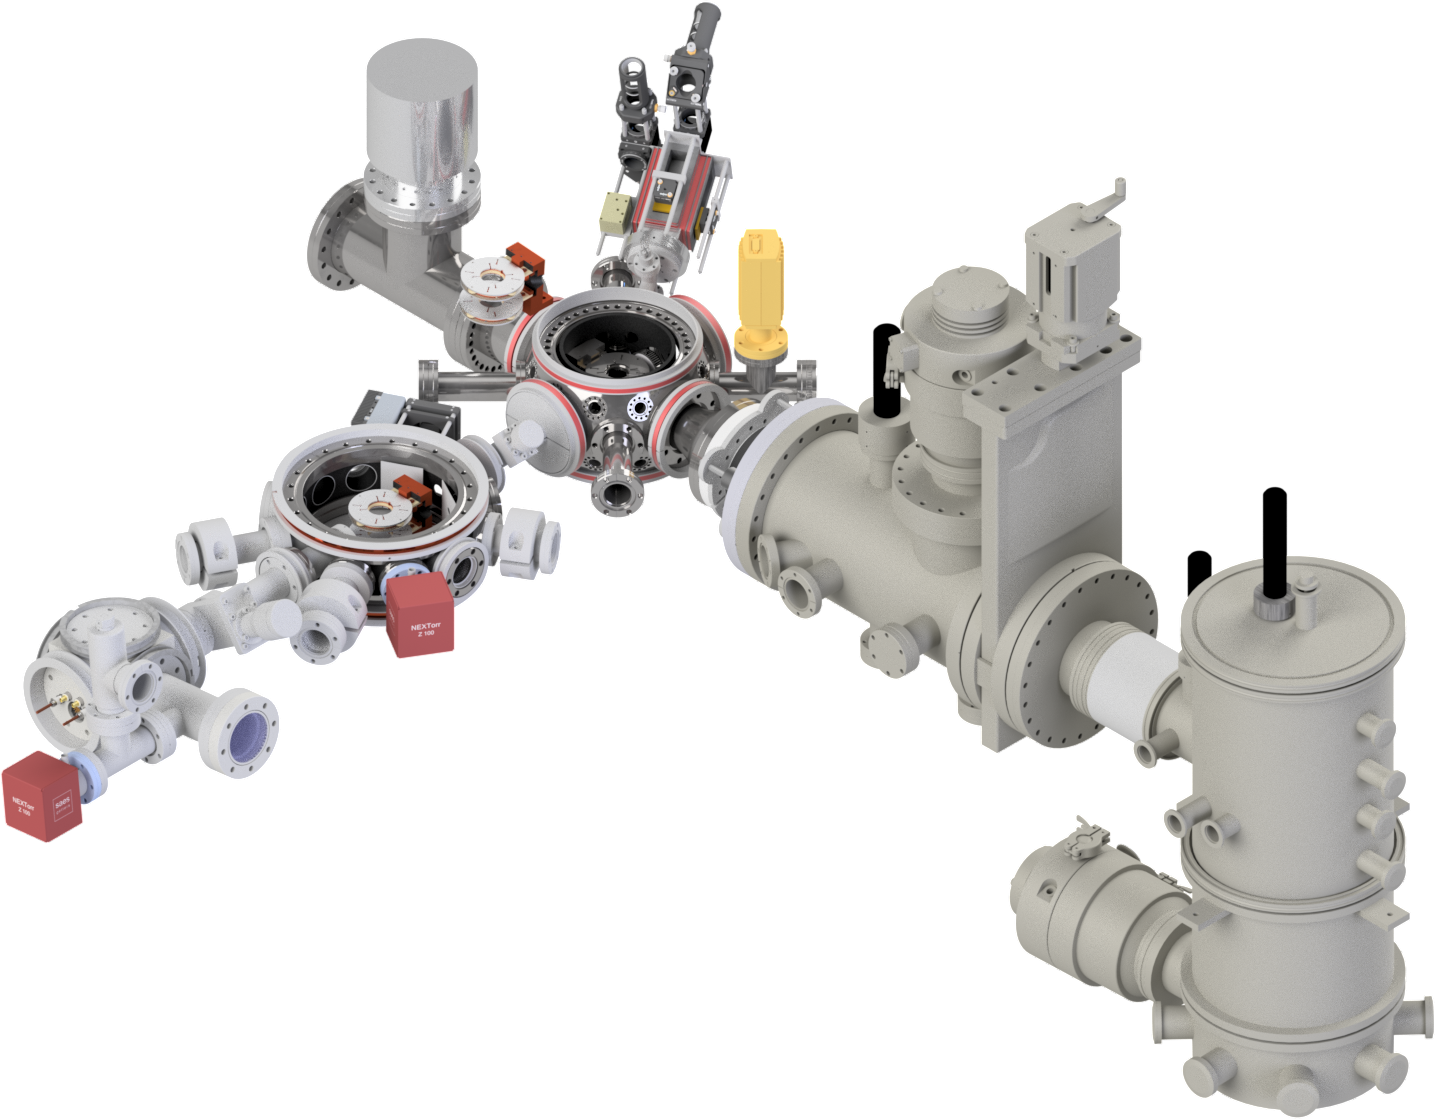
\includegraphics[width=0.7\textwidth]{figs/overview/apparatus_04_crp.png}
    \begin{tikzpicture}
      \node[anchor=south west,inner sep=0] (image)
{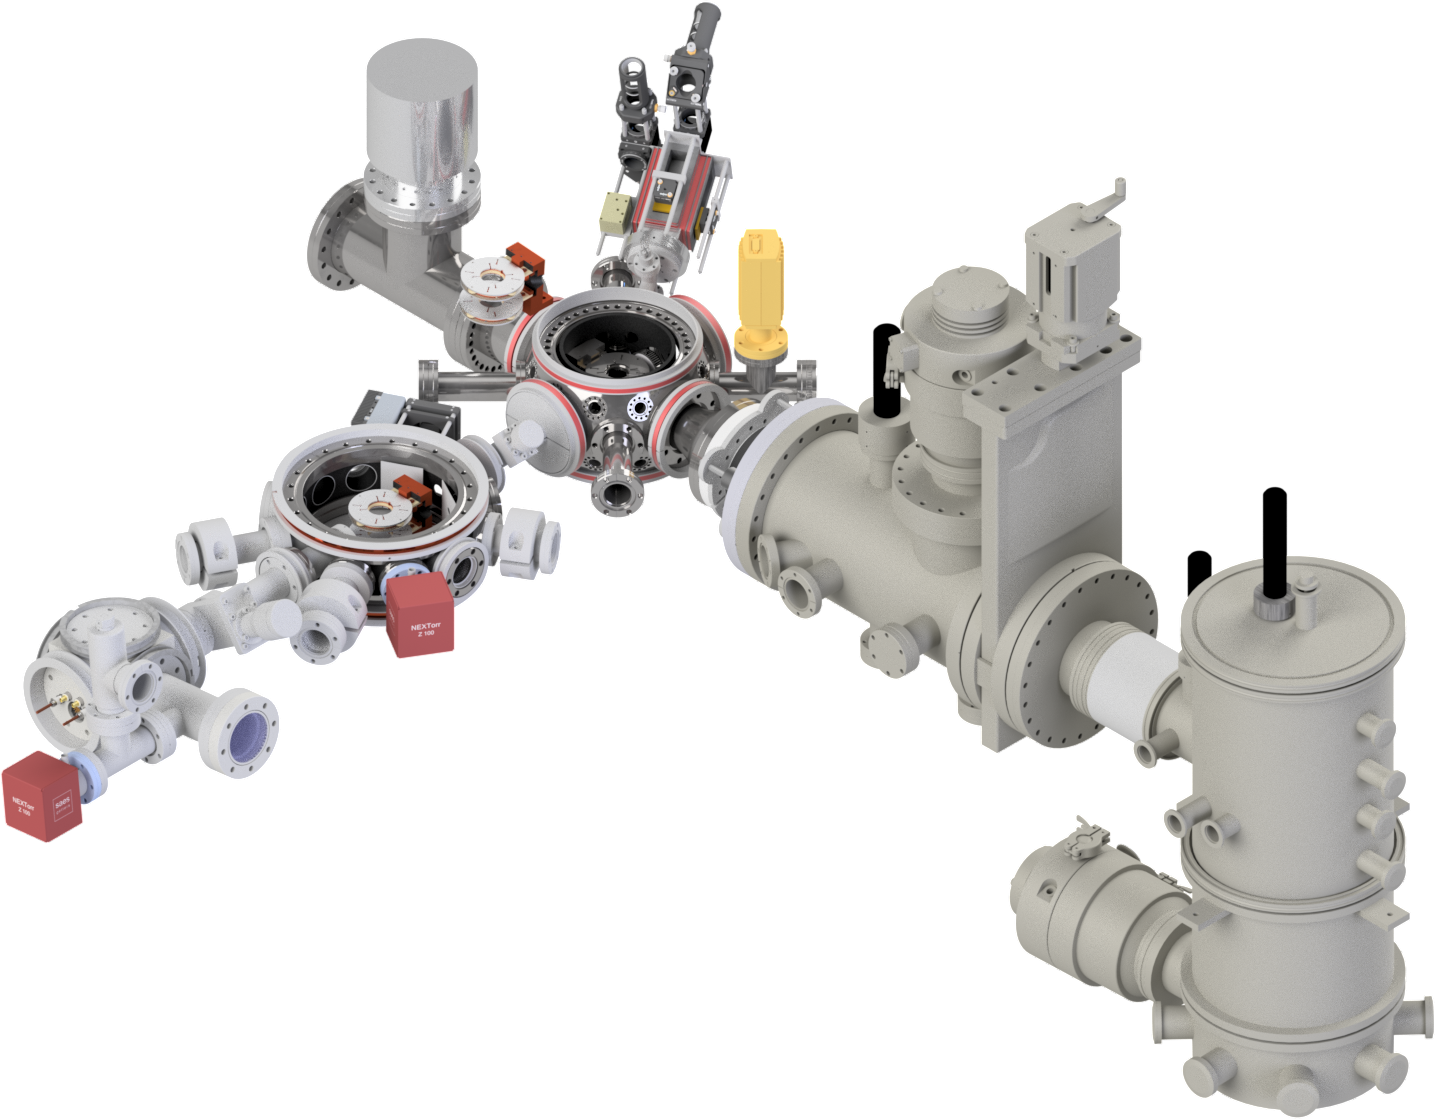
\includegraphics[width=0.8\textwidth]{figs/overview/apparatus_04_crp.png} };
      \begin{scope}[x={(image.south east)},y={(image.north west)}]
        \draw [-stealth] (0.45, 0.35) -- (0.45,0.52);
        \node[] at (0.46,0.3) {\small MOT chamber};
        \draw [-stealth] (0.18,0.23) -- (0.1, 0.3);
        \node[] at (0.21,0.2) {\small Chip chamber};
        \draw [-stealth] (0.15, 0.7) -- (0.2,0.63);
        \node[] at (0.12,0.72) {\small Tweezer chamer};
        \draw [-stealth] (0.7, 0.95) -- (0.52,0.85);
        \node[] at (0.72,0.99) {\small \Rb{} cell};
        \draw [-stealth] (0.95, 0.85) -- (0.8,0.7);
        \node[] at (0.97,0.89) {\small Slowing region};
        \draw [-stealth] (0.6, 0.2) -- (0.7,0.2);
        \node[] at (0.54,0.2) {\small Source};
      \end{scope}
    \end{tikzpicture}
  \caption{
    The \CaF{} experiment is shown along with the planned additional chip
    chamber. Not shown: external transport coils and transverse cooling region.}
  \label{overview:fig:vacuumsystem}
\end{figure}

At this point we note that the rotational stretched states of \CaF{} have been
demonstrated to have exceptionally long lifetimes in a macroscopic magnetic
trap~\cite{}. For this reason it was decided that using such traps would be
preferable to the electrostatic traps suggested in \inlineref{Andre2006}. This
has the additional problem of avoiding the need to transfer from a magnetic
trap to an electostatic one. This problem of loading is one that has been
similarly addressed for atom chips. For example \inlineref{} \cm{Ott paper?}
have transferred \cm{from a similar transport trap to ours?} into a chip trap,
via a macroscopic U-trap that is aligned with the chip. This makes it easier to
align the MTT and the chip trap.

From here it is a question of transferring a cloud of molecules from high above
the surface into a \SI{10}{\micro\meter} scale trap. Such a procedure is
non-tirival, and is the main subject of chapter~\ref{sim}. However it is
apparent from the literature that directly transferring from the macroscopic
% TODO Should be able to cite lots here
trap to the microscopic is highly inefficient~ \cite{}.
%
Instead, it is generally preferred to have a series of traps of decreasing
size. For magnetic traps, the width of the wires should decrease, so that the
molecules remain \cm{highly localised around the trap centre} throughout
loading.

Given that at this point we have free reign to design our series of traps, we
suggest that a \cm{Z trap is preferable to a U trap because of spin-flip
(Majorana) losses...}


\section{Design choices}
% TODO Maybe a better name for this 

\cm{
%
Everything below here is what was in the fab chapter before (I think...) Need
to rework it to fit more with the above. Maybe integrate entirely with the prev
section...
%
  \begin{itemize}
    \item Load with big U wire under chip
    \item Current and mw delivery by subchip (? this is a detail)
    \item Present design
  \end{itemize}
}




The chip experiment will integrate into this setup as shown in
\myfigref{overview:fig:vacuumsystem}, an additional chamber will be mounted
further downstream of the transport stage, so that molecules can be brought
straight through the tweezer chamber from the collisions chamber.  Since the
molecules will be brought into the chamber inside magnetic trap, we propose to
transfer them gradually into other magnetic traps formed on the chip.
%
Not only does this take advantage of the known, long-lived \CaF{} states in the
trap~\cite{WilliamsMagnetic2018}, but it allows us to follow the well-trodden
path of magnetic trapping near a chip, as has been outlined in previous
chapters.  The transfer to the chip will take the molecules through a series of
magnetic traps of decreasing size until they are in the smallest trap, similar
to what has previously been done in atom chips \cite{Reichel1999} or for
guiding molecules near surfaces \cite{Meek2009}

The chip will be held in its chamber recessed in a PCB used for power (and
later microwave) delivery. We use an aluminium-core PCB to ensure good heat
conduction away from the chip and we refer to it as the subchip.  This is
attached to a large copper heatsink, which has a large U-wire built into it,
isolated from the rest of the copper by aluminium-nitride plates. The heatsink
connects to a flange equipped with a \cm{?} pin feedthrough for chip currents,
and two high-current feedthroughs to power the U-wire.

% TODO Ensure I go on to discuss the current drivers
% TODO confirm distance in this para
We refer to this entire device as the flange assembly, and it is shown in the
inset of \myfigref{overview:fig:vacuumsystem} and in
\mysubfigref{overview:fig:chipexperiment} It will be mounted so that the chip is
\SI{3}{\milli\meter} away from the transport axis and facing the floor,
allowing us to trap and then drop the molecules for imaging.  External magnetic
coils will provide the bias fields, and currents will be provided by drivers
discussed in \cm{a later chapter.} {a}.

\begin{figure}[ht]
  \centering
  \begin{subfigure}[b]{0.45\textwidth}
    \includegraphics[width=\textwidth]{figs/chip_pic_crop.png}
    \caption{}
  \end{subfigure}
  \hspace{1cm}
  \begin{subfigure}[b]{0.45\textwidth}
    \centering
    %\includegraphics[width=\textwidth]{figs/chip_present2.pdf}
    \begin{overpic}[abs, width=\textwidth]{figs/chip_present4.pdf}
      \put(10, 160){\small (i)}
      \put(60, 160){\small(ii)}
      \put(175, 60){\small(iv)}
      \put(110, 137){\small(iii)}
      \put(70, 90){\small \SI{20}{\micro\meter}}
      \put(112, 93){\small\SI{10}{\micro\meter}}
      \put(8, 42){\small $\mathrm{Z_0}$}
      \put(8, 10){\small $\mathrm{Z_1}$}
      \put(8, 200){\small $\mathrm{Z_2}$}
    \end{overpic}
    \caption{}
  \end{subfigure}
  \caption{
    In (a) we have the chip assembly fully constructed, with a view of the
    aluminium-core PCB (subchip) for current delivery. Note also the polyimide
    bushings to electrically isolate the retaining screws from the surface. The
    microwave feedthroughs remain disconnected. In (b) we show a schematic of
    the chip features, with the scaling exaggerated for visibility. The three
    overlapping Z-wires are shown and labeled. The gaps between the wires are
    highlighted.
    %
    Toward the left (i) is the
    electroplating connection pad and various features used for
    characterisation (ii). On Z2 it is possible to see several small pads used
    as anchors, to secure the thin wire to the substrate.  The axis of the
    $\mathrm{Z1}$ wire is labeled for reference (iii) and the other wires are
    similar. All of the above features  will be discussed further in
    chapter~\ref{fab}. The crest of Imperial College London (iv) is also
    included.}
  \label{overview:fig:chipexperiment}
\end{figure}

% TODO Check what these equations that I use actually are and where they go. I
% think the current wording might basically be the same equation twice...
The first stage of the magnetic transfer is to take the molecules from the MTT
to the large U-wire embedded in the heat sink.  The idea is to use this as a
deep, macroscopic trap that is well-aligned with the chip by virtue of being
built into the assembly, and can be easily aligned with the MTT, similarly to
other experiments such as \inlineref{Ott2001}.  Since it is under the chip, it
will of course be further from the molecule cloud than the other wires, hence
more current will be required to create a deep trap (as per
equations~\ref{intro:eq:trapbias} and~\ref{intro:eq:trapdepth}). The current is
limited to \SI{100}{\ampere} by the vacuum feedthroughs, allowing for a trap of
depth around \SI{2}{\milli\kelvin} by equation \cm{ref. earlier chapter}.

Once loaded into the U-trap, the molecules will be transferred through the
Z-wire traps on the chip. Each Z-wire should be sufficiently
large to maintain the currents required to form a trap at height $z$ below the
trap, whilst having a width and height  $w, h \ll z$ so that that the current
is highly localised compared to the cloud size.  This follows the widely-made
assumption in the literature that the trapping currents are carried by wires
which are infinitesimally small compared to the length scale of the trap
~\cite{2011Ac}.

% TODO Make sure that this link to fab chapter is ok
In the case of the first Z-wire, the molecules are still \SI{3}{\milli\meter}
away from the trapping wire. If we demand a trap depth of
$k_B\times\SI{1}{\milli\kelvin}$, then we will require a trapping current of
\SI{30}{\ampere} to form a trap of this depth.  We will discuss in
chapter~\ref{fab} that the maximum wire height that can reliably be fabricated
is \SI{5}{\micro\meter}, and we expect that the wires will be able to carry a
maximum current density of \SI{6E10}{\ampere\per\meter\squared}, as was found
for a similar chip design in \inlineref{Treutlein2008}. The Z-wire will
therefore have a width $w=\SI{200}{\micro\meter}$. Other wire parameters are
shown in \mytableref{overview:table:wires}.

The axial length of the wires also decreases to gradually reduce the size of
the trapped cloud in the $x$ direction. An exaggerated schematic of the wire
layout is shown in \myfigref{overview:fig:chipexperiment} and further details are
outlined in \mytableref{overview:table:wires}. All wires have been designed to
carry twice the current that is required in the loading scheme, so that there
is sufficient headroom for further experiments, and to reduce risk of
accidental damage to the chip during normal operation.

% TODO Maybe need more detail here
\begin{table}
  \centering
\begin{tabular}{lrrrrr}
  Name & Axis length (\si{\milli\meter}) & Width (\si{\micro\meter})& $I_\text{max}$ & Trap height (\si{\micro\meter}) \\
 \hline
  U & 16 & N/A& 100 & 3000\\
  $\mathrm{Z0}$ & 12 & 200& 60& $3000\rightarrow1000$ \\
  $\mathrm{Z1}$ &  6 & 20& 6& $1000\rightarrow100$ \\
  $\mathrm{Z2}$ &  2 & 2& 0.6& $100\rightarrow10$ \\
 \hline
\end{tabular}
  \caption{Details on the wire dimensions, maximum current, and desired
  trapping heights. The wire design is shown in
  \mysubfigref{overview:fig:chipexperiment}{c}. Note that the U-wire current is
  limited by vacuum feedthroughs and not by the maximum current calculated by
  the wire dimensions.  The maximum currents have been designed for use at only
  50\% of their potential maximum ($I_\text{max}$).
  }
  \label{overview:table:wires}
\end{table}

Each Z-trap will begin trapping at one height before the bias field is
increased to bring the trap centre closer to the surface (as per
% TODO back to link
%\myeqref{intro:eq:trapbias}
\cm{reference eqn. $B = \mu_0 I / (2\pi h)$}
).  To distinguish between the two trap stages for
each wire, we label them $\mathrm{ZX_i}$ for the initial (higher) trap and
$\mathrm{ZX_f}$ for the final (lower) trap, with $\mathrm{ZX}$ corresponding to
the wire labels in \mytableref{overview:table:wires}.

In order to incorporate microwave guides onto the chip. This can be
accomplished by adding an insulating layer on top of the wires, on to which we
can fabricate coplanar waveguides~\cite{1127105}. The flange has been designed
with microwave feedthroughs, so that microwaves can be launched onto the
subchip and carried to the chip via coplanar waveguides \cm{to be discussed in
a later chapter}.

Having broadly outlined the experiment, the rest of this chapter will justify
the design of the trapping wires by means of simulation and analysis
of the trapping potentials.

